% Federates, HELICS topics and the operating layer of one experiment.
\documentclass[border=2pt]{standalone}
\usepackage{tikz}
\usetikzlibrary{arrows.meta,positioning,fit,calc}
\begin{document}
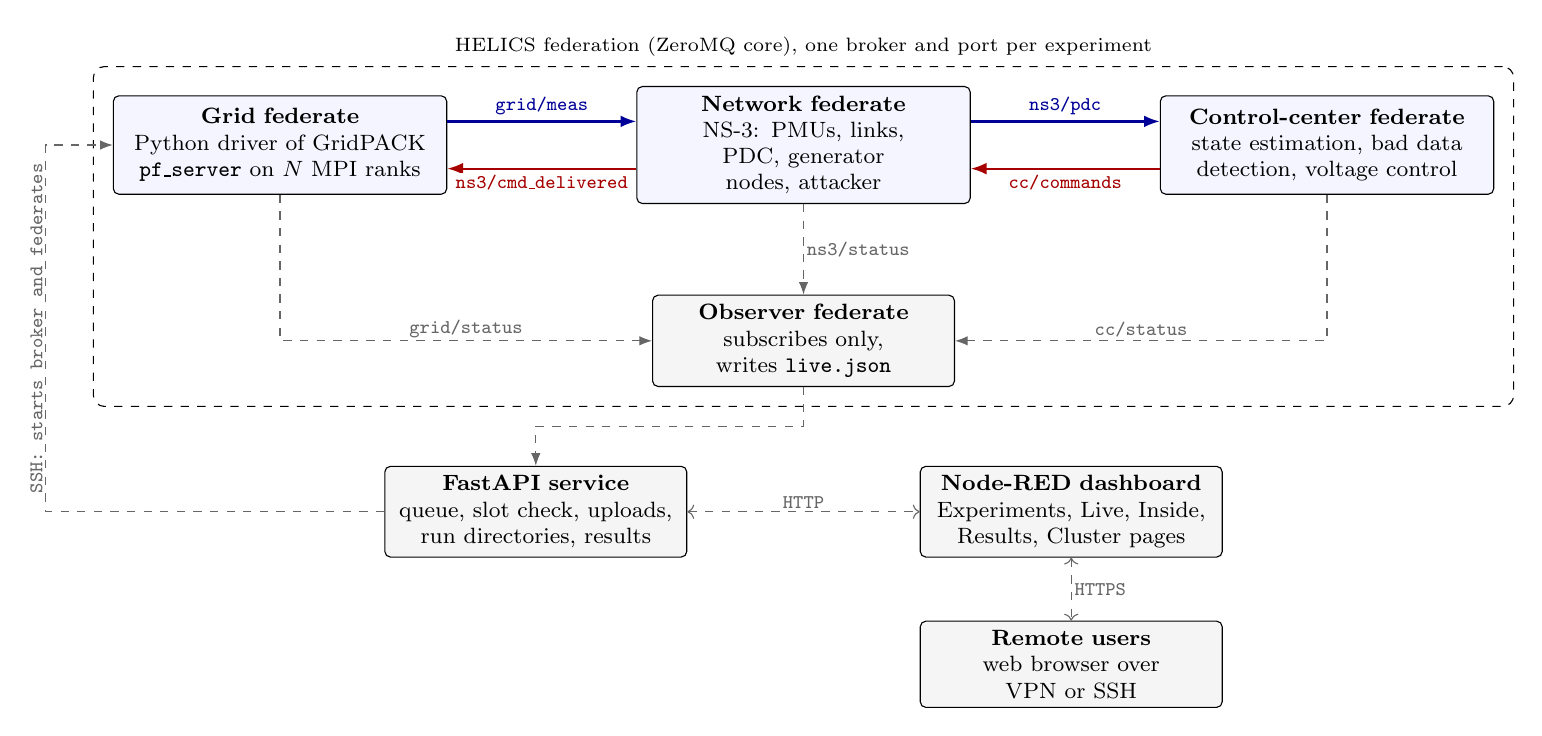
\begin{tikzpicture}[
  font=\footnotesize,
  fed/.style={draw, rounded corners=2pt, align=center, minimum height=1.25cm, text width=4.0cm, fill=blue!4},
  aux/.style={draw, rounded corners=2pt, align=center, minimum height=0.9cm, text width=3.6cm, fill=gray!8},
  meas/.style={-{Latex[length=2mm]}, thick, blue!60!black},
  cmd/.style={-{Latex[length=2mm]}, thick, red!65!black},
  obs/.style={-{Latex[length=1.6mm]}, gray!80!black, dashed},
  lab/.style={font=\scriptsize\ttfamily, fill=white, inner sep=1pt}]
\node[fed] (grid) {\textbf{Grid federate}\\ Python driver of GridPACK\\ \texttt{pf\_server} on $N$ MPI ranks};
\node[fed, right=2.4cm of grid] (ns3) {\textbf{Network federate}\\ NS-3: PMUs, links,\\ PDC, generator nodes, attacker};
\node[fed, right=2.4cm of ns3] (cc) {\textbf{Control-center federate}\\ state estimation, bad data\\ detection, voltage control};
\draw[meas] ([yshift=3mm]grid.east) -- node[lab, above=1pt] {grid/meas} ([yshift=3mm]ns3.west);
\draw[cmd] ([yshift=-3mm]ns3.west) -- node[lab, below=1pt] {ns3/cmd\_delivered} ([yshift=-3mm]grid.east);
\draw[meas] ([yshift=3mm]ns3.east) -- node[lab, above=1pt] {ns3/pdc} ([yshift=3mm]cc.west);
\draw[cmd] ([yshift=-3mm]cc.west) -- node[lab, below=1pt] {cc/commands} ([yshift=-3mm]ns3.east);
\node[aux, below=1.15cm of ns3] (obsv) {\textbf{Observer federate}\\ subscribes only, writes \texttt{live.json}};
\draw[obs] (grid.south) |- node[lab, pos=0.75, above] {grid/status} (obsv.west);
\draw[obs] (ns3.south) -- node[lab, right] {ns3/status} (obsv.north);
\draw[obs] (cc.south) |- node[lab, pos=0.75, above] {cc/status} (obsv.east);
\node[draw, dashed, rounded corners, fit=(grid)(ns3)(cc)(obsv), inner sep=7pt, label={[font=\scriptsize]above:HELICS federation (ZeroMQ core), one broker and port per experiment}] (fedbox) {};
\node[aux, below=1.0cm of obsv, xshift=-3.4cm] (api) {\textbf{FastAPI service}\\ queue, slot check, uploads,\\ run directories, results};
\node[aux, below=1.0cm of obsv, xshift=3.4cm] (nr) {\textbf{Node-RED dashboard}\\ Experiments, Live, Inside,\\ Results, Cluster pages};
\node[aux, below=0.8cm of nr] (user) {\textbf{Remote users}\\ web browser over VPN or SSH};
\draw[obs, <->] (api) -- node[lab, above] {HTTP} (nr);
\draw[obs, <->] (nr) -- node[lab, right] {HTTPS} (user);
\draw[obs] (obsv.south) -- ++(0,-0.5) -| (api.north);
\draw[obs] (api.west) -- ([xshift=-6mm]fedbox.west |- api.west) |- node[lab, pos=0.25, sloped, above] {SSH: starts broker and federates} (grid.west);
\end{tikzpicture}
\end{document}
